%==============================================================================
%  Application of Fourier Neural Operator as Autoregressive Neural Surrogate
%  for Geothermal Simulation
%
%  Springer Nature template (sn-jnl.cls v3.1, Dec 2024).
%  Author-year, Math & Physical Sciences reference style (sn-mathphys-ay).
%==============================================================================
\documentclass[pdflatex,sn-mathphys-ay]{sn-jnl}
%------------------------------- Packages -------------------------------------
% NOTE: sn-jnl already loads geometry, natbib (per the documentclass option),
% and hyperref internally -- do NOT load them here or LaTeX will clash.
% Fonts/encoding are handled by the class as well.

\usepackage{amsmath,amssymb,amsfonts,bm}
\usepackage{mathtools}
\usepackage{siunitx}              % \SI{640}{\meter}, units
\DeclareSIUnit{\darcy}{D}         % permeability: \si{\milli\darcy} -> mD
\usepackage{graphicx}
\usepackage{booktabs}             % \toprule \midrule \bottomrule
\usepackage{multirow}
\usepackage{xcolor}
\usepackage{tikz}
\usetikzlibrary{positioning,arrows.meta,fit,backgrounds,calc,shapes.misc,shapes.geometric}
\usepackage{algorithm}
\usepackage{algpseudocode}        % training-loop pseudocode
% cleveref must come after the class's hyperref (it does); drives all \cref's.
\usepackage[capitalize,noabbrev]{cleveref}
% The class ships uncolored links for submission. Uncomment for draft-time
% colored links:
% \hypersetup{colorlinks=true,allcolors=blue}

%---------------------------- Custom commands ---------------------------------
% Notation helpers -- adjust to taste.
\newcommand{\svec}{\mathbf{u}}            % reservoir state field
\newcommand{\action}{\mathbf{a}}           % well-control action
\newcommand{\model}{\mathcal{G}_\theta}    % learned operator
\newcommand{\R}{\mathbb{R}}
\DeclareMathOperator{\diag}{diag}

% Editorial markers -- delete before submission.
\newcommand{\todo}[1]{\textcolor{red}{[\textbf{TODO:} #1]}}
\newcommand{\note}[1]{\textcolor{blue}{[\emph{#1}]}}

%---------------------- TikZ palette + styles (architecture fig) --------------
\definecolor{cGlobal}{HTML}{2C5F8A}   % global spectral branch
\definecolor{cLocal}{HTML}{2E7D5B}    % local patch branch
\definecolor{cHF}{HTML}{C25A1A}       % high-frequency branch
\definecolor{cCond}{HTML}{6A4C93}     % action / AdaLN conditioning
\definecolor{cAux}{HTML}{0F7B7B}      % auxiliary head
\definecolor{cLift}{HTML}{37474F}     % lifting / projection
\tikzset{
  >={Latex[length=2mm]},
  font=\footnotesize,
  io/.style={draw=none, font=\small\bfseries, text=black!80, align=center},
  blk/.style={rounded corners=2pt, draw=#1!70, fill=#1!10, text=black!85,
              line width=0.7pt, align=center, inner sep=4pt, minimum height=8mm},
  blk/.default=cLift,
  stack/.style={rounded corners=2pt, draw=cGlobal!70, fill=cGlobal!8,
                line width=0.7pt, align=center, inner sep=4pt},
  op/.style={circle, draw=black!70, fill=black!4, line width=0.7pt,
             inner sep=0pt, minimum size=5.5mm, font=\small},
  arr/.style={->, line width=0.7pt, draw=black!65},
  arrc/.style={->, line width=0.7pt, draw=cCond!75, densely dashed},
  zlabel/.style={font=\scriptsize\itshape, text=black!60},
  panel/.style={rounded corners=3pt, draw=black!45, densely dashed,
                line width=0.8pt, fill=black!2, inner sep=7pt},
  bgbox/.style={rounded corners=3pt, draw=black!20, fill=black!2,
                line width=0.6pt, inner sep=8pt},
}

%==============================================================================
\begin{document}

%------------------------------- Front matter ---------------------------------
\title[FNO Surrogate for Geothermal Simulation]{Application of Fourier Neural
       Operator as an Autoregressive Neural Surrogate for Geothermal Simulation}

\author*[1]{\fnm{Thanh} \sur{Nguyen}}\email{nguyentuthanhdn@gmail.com}
% \author[1]{\fnm{First} \sur{Author}}\email{}   % \todo{co-authors}

\affil*[1]{\orgdiv{\todo{Department}}, \orgname{\todo{Organization}},
  \orgaddress{\city{\todo{City}}, \country{\todo{Country}}}}

%------------------------------- Abstract -------------------------------------
\abstract{%
Geothermal energy is a promising solution to the worldwide growing demand for
clean energy. Operating geothermal reservoirs requires careful engineering
decisions, often involving repeated numerical simulation runs to identify
optimal well controls. The expensive computational cost of these simulations has
motivated interest in data-driven surrogate models, where a neural network is
trained on simulation-generated data and acts as a proxy for future engineering
workflows. Building such neural surrogates is a challenging problem: we want the
model's predictions to closely match the simulator outputs, and to maintain that
accuracy autoregressively into the future, all while training on as little data
as possible. In this work, we propose two 3D geothermal datasets to evaluate our
surrogate model: one with homogeneous and one with heterogeneous porosity and
permeability fields. Training on only 300 trajectories, our adapted Fourier
Neural Operator with several architectural and training modifications achieves
\SI{0.1}{\percent} relative error on 3D pressure and temperature predictions, and
remains stable autoregressively across 156 time steps.
}

\keywords{geothermal reservoir simulation, Fourier neural operator,
  surrogate modeling, autoregressive rollout, operator learning}

\maketitle

%============================== 1. Introduction ================================
\section{Introduction}
\label{sec:intro}

Numerical simulators have been used in geothermal reservoir management for a long
time, supporting engineering workflows such as history matching, well placement,
well-schedule optimization, uncertainty quantification, and production
forecasting. Non-isothermal simulators include SHEMAT, FEFLOW, OpenGeoSys,
ECLIPSE, and STARS, to name a few. While these tools differ in their
discretization strategies, the governing equations must still be linearized, and
the linear systems must be solved iteratively until convergence. This process
becomes increasingly expensive as spatial resolution, physical complexity, and
simulation duration grow. The cost is further amplified in engineering workflows
such as optimal well control, where the simulation must be run hundreds of times
to explore the decision space.

The prohibitive cost of repeated numerical runs has motivated growing interest in
data-driven surrogate models, where a neural network is trained on trajectories
generated by a simulator and serves as a fast proxy for iterative workflows.

\todo{state the gap / what is missing in prior work, then the contributions.}

\paragraph{Contributions.} In this work we:
\begin{itemize}
  \item release two 3D dual-porosity geothermal datasets (homogeneous and
        heterogeneous porosity/permeability) for benchmarking surrogate models;
  \item adapt the Local--Global Fourier Neural Operator (LoGlo-FNO) to 3D
        non-isothermal geothermal simulation with several architectural and
        training modifications;
  \item demonstrate \SI{0.1}{\percent} relative error and stable 156-step
        autoregressive rollouts while training on only 300 trajectories;
  \item \todo{ablations / additional contributions.}
\end{itemize}

%============================== 2. Related Work ================================
\section{Related Work}
\label{sec:related}

UNet-based models leverage convolutional encoders and decoders to learn
multiscale spatial features, making them a natural fit for grid-based simulation
data. Fourier Neural Operators (FNOs) and their variants approach the problem
from a different angle: grounded in the theory of learning mappings between
function spaces, they parameterize the solution operator directly in the
frequency domain, offering resolution-invariant learning with strong theoretical
foundations. Among these variants, the Local--Global Fourier Neural Operator
(LoGlo-FNO) extends the standard FNO by explicitly learning high-frequency
features through local convolutions alongside the global spectral modes,
addressing a well-known limitation of purely Fourier-based approaches. Transolver
generalizes the operator-learning paradigm further by attending over learned
physical states rather than fixed spatial positions, offering flexibility for
problems with complex geometries. Graph neural networks have also attracted
attention, as they naturally represent the connectivity between grid blocks in a
manner analogous to flux computation in discretized conservation laws.

Beyond architecture, training strategies also play a critical role in surrogate
model quality. Autoregressive surrogate models are prone to error accumulation
over long rollouts, and techniques such as the pushforward trick---which trains
the model on its own predictions rather than solely on ground-truth
inputs---have been shown to significantly improve temporal stability.

While the list above is far from exhaustive and the surrogate-modeling literature
continues to grow rapidly, these approaches represent the principal architectural
families relevant to our setting. In this work, we focus on architectures that
operate on structured 3D grids, which rules out graph-based methods due to the
prohibitive memory cost of constructing graphs over the large number of nodes in
our discretization. We therefore benchmark against UNet, FNO, and Transolver as
baselines, and build our primary model on the LoGlo-FNO architecture, introducing
several modifications to adapt it to 3D non-isothermal geothermal simulation.

%================================ 3. Methods ===================================
\section{Methods}
\label{sec:methods}

%---------------------------- 3.1 Dataset generation --------------------------
\subsection{Dataset Generation}
\label{sec:data}

We generated two datasets: one homogeneous in porosity and permeability, and a
heterogeneous counterpart. Each dataset contains 400 simulation runs, each
spanning 156 weekly timesteps, corresponding to three years of operation. Because
we use the dual-permeability (DUALPERM) setting in STARS, every run carries
separate matrix and fracture properties. The reservoir spans \SI{640}{\meter} in
width, \SI{320}{\meter} in length, and \SI{160}{\meter} in height, discretized
into $\SI{10}{\meter} \times \SI{10}{\meter} \times \SI{10}{\meter}$ cells, giving
$64 \times 32 \times 16 = 32{,}768$ cells in total. The wells are arranged in a
stacked inverted five-spot pattern, with 2 injectors and 7 producers, as shown in
\cref{fig:well-pattern}. The porosity, permeability, and remaining simulation
parameters are described in \cref{sec:rock}, and the 400 varying well schedules
shared across both datasets are described in \cref{sec:schedules}.

\begin{figure}[t]
  \centering
  % \includegraphics[width=0.6\textwidth]{figures/well_pattern.pdf}
  \todo{well pattern / domain figure}
  \caption{Stacked inverted five-spot well pattern (2 injectors, 7 producers)
           and reservoir domain.}
  \label{fig:well-pattern}
\end{figure}

%-------------------- 3.1.1 Porosity, permeability ----------------------------
\subsubsection{Porosity, Permeability, and Other Simulation Parameters}
\label{sec:rock}

For the homogeneous dataset, porosity and permeability are held constant across
the field (\cref{tab:homo-props}): the matrix has porosity 0.05 and permeability
\SI{0.1}{\milli\darcy}, while the fractures have porosity 0.005 and permeability
\SI{50}{\milli\darcy}.

For the heterogeneous dataset, we used unconditional Gaussian simulation to
generate 400 matrix porosity realizations and 400 fracture porosity realizations
(\cref{tab:hetero-props}). Both use omnidirectional variograms. The horizontal
variogram is spherical with 10 lags of \SI{10}{\meter}, \SI{150}{\meter} search
radius, range \SI{100}{\meter}, nugget 0.1, and sill 0.9. The vertical variogram
is spherical with 5 lags of \SI{10}{\meter} (one cell block each),
\SI{80}{\meter} search radius, range \SI{50}{\meter}, nugget 0.1, and sill 0.9.
Matrix porosity is drawn with mean 0.05 and variance $2.5 \times 10^{-5}$, and
fracture porosity with mean 0.005 and variance $1 \times 10^{-6}$. To ensure
every block sustains some flow, we clip matrix porosity to $[0.035, 0.065]$ and
fracture porosity to $[0.002, 0.008]$, corresponding to $\pm 3$ standard
deviations about each mean.

Permeability is then derived from porosity. Matrix permeability follows
\begin{equation}
  k_{\text{matrix}} = \exp\!\left(29.182291\,\phi - 4.017112\right)\ \si{\milli\darcy},
  \label{eq:k-matrix}
\end{equation}
which keeps matrix permeability within $[0.05, 0.12]\ \si{\milli\darcy}$, and
fracture permeability follows
\begin{equation}
  k_{\text{fracture}} = \exp\!\left(3.21888 + 0.536479\,
    \frac{\phi - \mu_\phi}{\sigma_\phi}\right)\ \si{\milli\darcy},
  \label{eq:k-fracture}
\end{equation}
which keeps fracture permeability within $[5, 125]\ \si{\milli\darcy}$. Both
datasets use a fracture spacing of \SI{2}{\meter}, averaging about 5 fractures per
cell block. These values were chosen so the simulation resembles a volcanic rock
(porosity 0.05, permeability \SI{0.1}{\milli\darcy}) that has been mildly
stimulated, mechanically or chemically---reflected in the dense fracturing and
the elevated fracture permeability between \SI{5}{} and \SI{125}{\milli\darcy}.

\begin{table}[t]
  \centering
  \caption{Homogeneous-dataset rock properties.}
  \label{tab:homo-props}
  \begin{tabular}{lcc}
    \toprule
                 & Matrix & Fracture \\
    \midrule
    Porosity          & 0.05  & 0.005 \\
    Permeability (mD) & 0.1   & 50    \\
    \bottomrule
  \end{tabular}
\end{table}

\begin{table}[t]
  \centering
  \caption{Heterogeneous-dataset geostatistical parameters.}
  \label{tab:hetero-props}
  \todo{fill variogram / distribution parameters table}
  \begin{tabular}{lcc}
    \toprule
                 & Matrix & Fracture \\
    \midrule
    Mean porosity     & 0.05 & 0.005 \\
    Variance          & $2.5\times10^{-5}$ & $1\times10^{-6}$ \\
    Clip range        & $[0.035, 0.065]$ & $[0.002, 0.008]$ \\
    \bottomrule
  \end{tabular}
\end{table}

%-------------------- 3.1.2 Well control schedules ----------------------------
\subsubsection{Well Control Schedules}
\label{sec:schedules}

We want our surrogate model to be robust and able to capture highly irregular and
chaotic physical dynamics. With this goal in mind, we randomly divide the 156
timesteps into chunks of 2, 3, or 4 weeks. Within each chunk, we sample the rate
for each injector from a uniform distribution between \SI{500}{} and
\SI{3000}{\cubic\meter\per\day}. For the producers, we scale the sum of all
injector rates by a scalar drawn from a uniform distribution between 0.92 and
1.05, ensuring the producers do not draw the reservoir down too quickly, and then
randomly allocate this scaled total across the 7 producers. To make the dynamics
even more irregular, every injector and producer has a \SI{10}{\percent} chance of
shutting in during each chunk, where its rate is set to zero and the remaining
well rates are adjusted accordingly. This procedure yields highly irregular
well-control schedules, which in turn drive complex, chaotic reservoir dynamics to
test our surrogate model's ability to learn and generalize with limited data.

%---------------------------- 3.2 Problem formulation -------------------------
\subsection{Problem Formulation}
\label{sec:problem}

  After running the 400 simulations for each dataset, we extract the pressure and
  temperature fields at weekly intervals from the STARS output (.sr3) files, giving
  156 time steps per trajectory. Each field has four channels: matrix temperature,
  fracture temperature, matrix pressure, and fracture pressure. For each dataset, 
  we split the 400 trajectories into 300 for training and 100 for testing.

  Since we extract pressure and temperature fields at weekly intervals, we can view our learning
  problem as an Euler discretization of the reservoir dynamics, where an operator 
  $\model$ models the per-step rate of change,
  \begin{equation}
    \frac{\svec_{t+1} - \svec_t}{\Delta t} = \model(\svec_t, \action_t).
    \label{eq:euler}
  \end{equation}
  Taking a unit step size $\Delta t = 1$,
  \begin{equation}
    \svec_{t+1} = \svec_t + \model(\svec_t, \action_t),
    \label{eq:update}
  \end{equation}
  where $\svec_t = [T_{\text{matrix}}, T_{\text{fracture}}, P_{\text{matrix}},
  P_{\text{fracture}}]$ is the four-channel state field at time $t$, $\model$ is the
  surrogate model, and $\action_t$ is the well-control action. The action is encoded
  as a $16 \times 64 \times 32$ tensor that holds each well's rate at its perforated
  cells (layers 2--13, see Table~1) and zero elsewhere. We concatenate it with a
  second tensor of the same shape: a binary mask that is 1 at active perforated cells
  and 0 at shut-in cells. This formulation treats the reservoir dynamics as Markov: the next state
  $\svec_{t+1}$ is fully determined by the current state $\svec_t$ and the current
  action $\action_t$, with no dependence on earlier history. This assumption is well
  grounded in how the data are generated. The governing mass and energy balance
  equations are first order in time, so the instantaneous rate of change of the state
  depends only on the present state and the present well controls. The numerical
  simulator inherits this structure: it advances each time step by solving an implicit
  system assembled solely from the state at time $t$ and the controls applied over the
  step. The surrogate therefore only needs to learn this single-step update, and
  conditioning on additional past states would be redundant.

  Beyond predicting the next state $\svec_{t+1}$, the same setup can be extended to
  learn any derived quantity of interest. Formally, given the current and next states
  we predict a target vector
  \begin{equation}
    \mathbf{q}_t = \mathcal{H}_\psi(\svec_t, \svec_{t+1}) = \mathcal{H}_\psi\!\left(\svec_t, \svec_t + \model(\svec_t, \action_t)\right),
    \label{eq:aux}
  \end{equation}
  where $\mathcal{H}_\psi$ is a separate auxiliary head. The choice of $\mathbf{q}_t$
  is problem-specific and can be set to whatever a downstream workflow needs. Here we
  let $\mathbf{q}_t$ be the bottomhole pressure at each of the 9 wells and the energy
  production rate at each of the 7 producers (16 values in total).
  

%---------------------------- 3.3 Model architecture --------------------------
\subsection{Model Architecture}
\label{sec:arch}

As discussed in \cref{sec:related}, LoGlo-FNO is well suited to our 3D
non-isothermal data because it captures both the global trends and the local
high-frequency features of the fields. We view the well-control action at each
time step as a conditioning signal that modulates the reservoir dynamics. Under
this view, rather than concatenating the action with the state and feeding both
through LoGlo-FNO, it is more natural to learn a rich representation of the action
and use it to modulate the hidden state, yielding a more flexible and expressive
model. To this end, we add a modulation encoder that maps the
action---together with the porosity and permeability fields in the heterogeneous
dataset---to per-block parameters $\gamma$ and $\beta$. These parameters share the
shape of the hidden state and modulate it through adaptive LayerNorm
(AdaLN)~\todo{FiLM/AdaLN citation},
\begin{equation}
  \mathrm{AdaLN}(z; \gamma, \beta) = \mathrm{LayerNorm}(z) \odot (1+\gamma) + \beta,
  \label{eq:adalin}
\end{equation}
where $z$ is the hidden state, $\mathrm{LayerNorm}$ normalizes $z$ over the
channel dimension, $\gamma$ and $\beta$ are per-layer modulation parameters produced by
the encoder, and $\odot$ denotes element-wise multiplication. We show empirically
in \cref{sec:ablations} that conditioning the hidden state through this modulation
encoder outperforms directly concatenating the action with the state.


\begin{figure}[tb]
  \centering
  % Bleed symmetrically into both margins: image is wider than \textwidth but
  % the surrounding \makebox keeps the caption at normal text width.
  \makebox[\textwidth]{%
    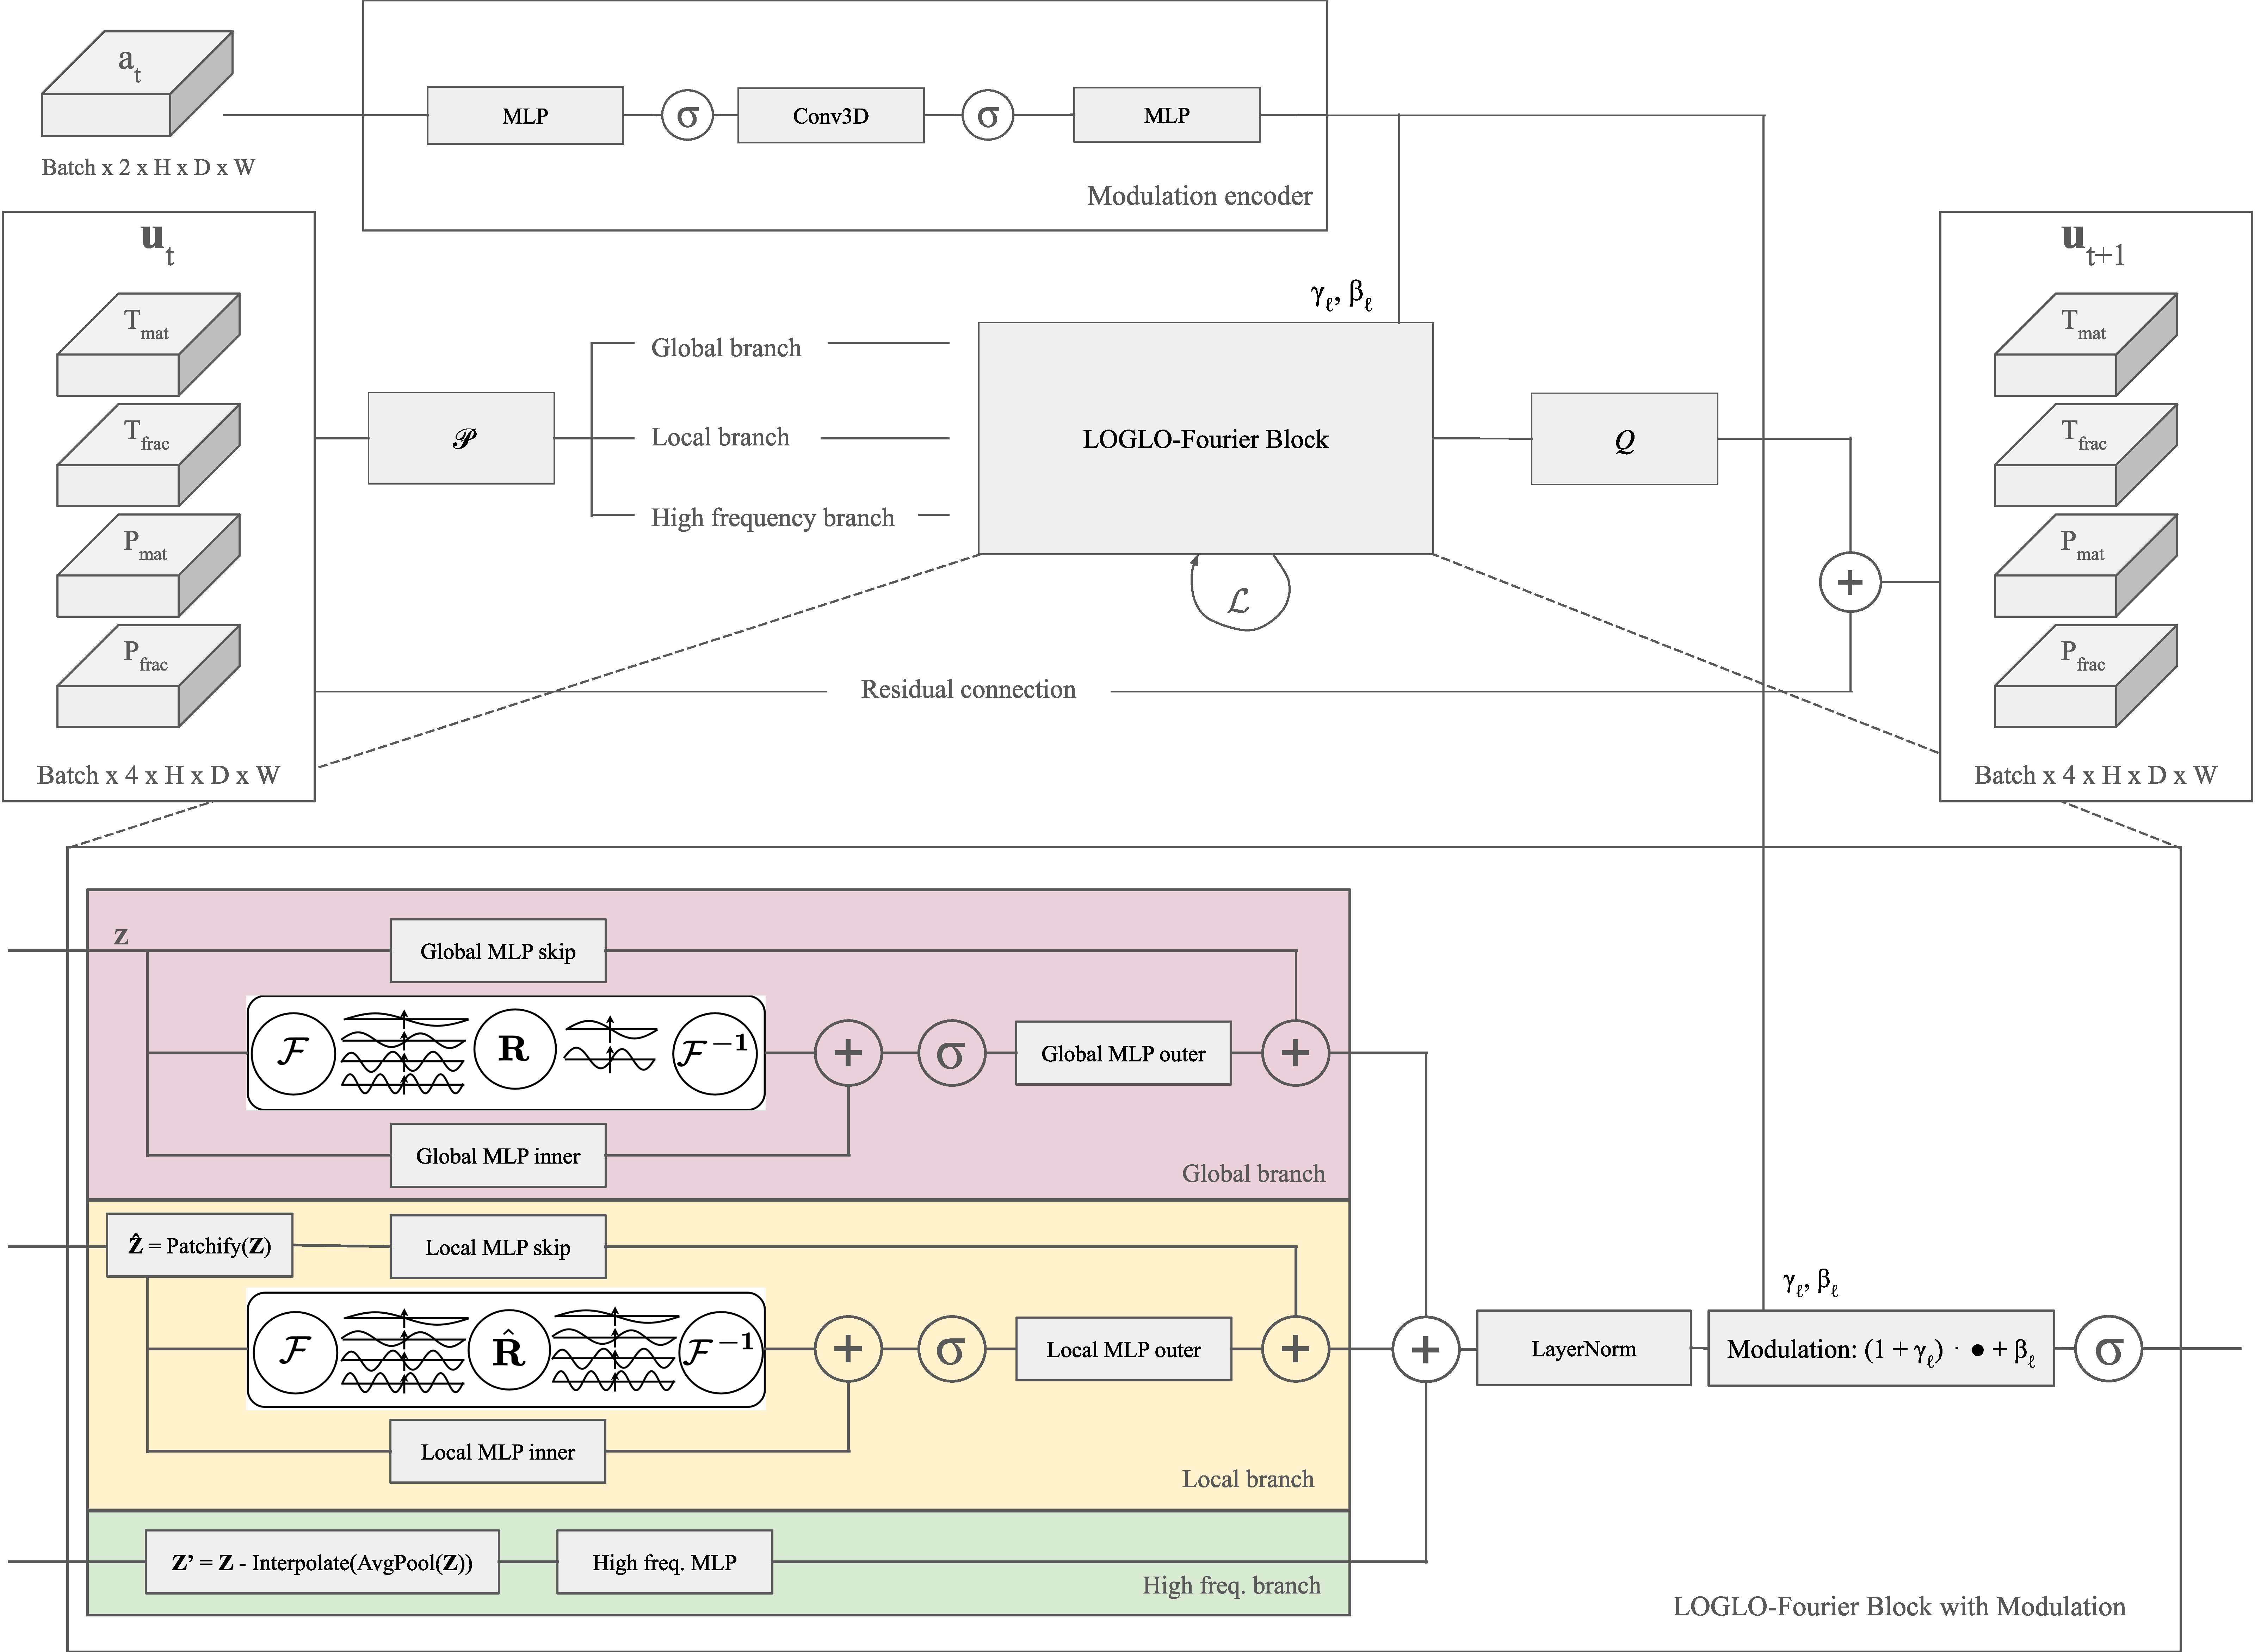
\includegraphics[width=\dimexpr\textwidth+1.6in\relax]{figures/loglofno_architecture.pdf}}
  \caption{TBD}
  \label{fig:arch}
\end{figure}

%---------------------------- 3.4 Training ------------------------------------
\subsection{Training}
\label{sec:training}

\todo{Pushforward training (unroll $k$ AR steps, $k$ schedule), multi-loss
objective (weighted MSE, H1/Sobolev, radial-binned spectral, mass-balance-equation
residual, mean-field pressure, auxiliary MSE), adaptive input noise, EMA, LR
schedule (linear warmup $\to$ cosine decay), fp32 training.}

\begin{algorithm}[t]
  \caption{Pushforward autoregressive training (sketch)}
  \label{alg:training}
  \begin{algorithmic}[1]
    \State \todo{pseudocode for the training loop}
  \end{algorithmic}
\end{algorithm}

%============================== 4. Experiments =================================
\section{Experiments}
\label{sec:experiments}

\subsection{Experimental Setup}
\label{sec:setup}
\todo{Hardware (H100), optimizer, batch size, epochs, seeds, normalization
(min--max; log1p for energy rate), reproducibility details.}

\subsection{Baselines}
\label{sec:baselines}
\todo{UNet3D, FNO, Transolver configurations and the experiment matrix.}

\subsection{Evaluation Metrics}
\label{sec:metrics}
\todo{Relative $L_2$ / per-channel relative error, rollout error vs.\ horizon,
spectral error, auxiliary (BHP, energy rate) error.}

%================================ 5. Results ===================================
\section{Results}
\label{sec:results}

\subsection{Homogeneous Reservoir}
\label{sec:results-homo}
\todo{quantitative table + rollout-error-vs-time plot + qualitative fields.}

\begin{table}[t]
  \centering
  \caption{Test-set accuracy on the homogeneous dataset (lower is better).}
  \label{tab:results-homo}
  \begin{tabular}{lcccc}
    \toprule
    Model & Rel. $L_2$ (\%) & 156-step Rel. $L_2$ (\%) & Aux. error & Params \\
    \midrule
    UNet3D     & & & & \\
    FNO        & & & & \\
    Transolver & & & & \\
    LoGlo-FNO (ours) & & & & \\
    \bottomrule
  \end{tabular}
\end{table}

\subsection{Heterogeneous Reservoir}
\label{sec:results-hetero}
\todo{same structure as homogeneous; emphasize generalization across static
fields.}

\subsection{Ablations}
\label{sec:ablations}
\todo{pushforward on/off, individual loss terms, EMA, noise injection,
local-global branches.}

%================================ 6. Discussion ================================
\section{Discussion}
\label{sec:discussion}
\todo{Interpretation, failure modes, limitations (data regime, single reservoir
geometry), and implications for well-control optimization.}

%================================ 7. Conclusion ================================
\section{Conclusion}
\label{sec:conclusion}
\todo{Summarize contributions and outline future work.}

%---------------------------- Back matter -------------------------------------
\backmatter

\bmhead{Acknowledgements}
\todo{funding, compute (DRAC/Fir cluster), collaborators.}

\section*{Declarations}
\begin{itemize}
  \item Funding: \todo{}
  \item Competing interests: \todo{}
  \item Data availability: \todo{links to datasets}
  \item Code availability: \todo{link to repository}
\end{itemize}

% The bibliography style is selected by the documentclass option
% (sn-mathphys-ay) -- do not use \bibliographystyle here.
\bibliography{references}

\end{document}


